\documentclass{article} % For LaTeX2e
\usepackage{nips14submit_e,times}
\usepackage{hyperref}
\usepackage{url}
\usepackage[utf8]{inputenc}
\usepackage{amsmath}
\usepackage{graphicx} 

\title{Analyzing Movie Character Networks Using Random Graph Models}


\author{
Vinayak Rai \\
Humanities \& Social Sciences \\
Indian Institute of Technology Roorkee\\
Roorkee, Haridwar 247667 \\
v\_rai@hs.iitr.ac.in\\
}

% The \author macro works with any number of authors. There are two commands
% used to separate the names and addresses of multiple authors: \And and \AND.
%
% Using \And between authors leaves it to \LaTeX{} to determine where to break
% the lines. Using \AND forces a linebreak at that point. So, if \LaTeX{}
% puts 3 of 4 authors names on the first line, and the last on the second
% line, try using \AND instead of \And before the third author name.

\newcommand{\fix}{\marginpar{FIX}}
\newcommand{\new}{\marginpar{NEW}}

\nipsfinalcopy % Uncomment for camera-ready version

\begin{document}


\maketitle

\begin{abstract}
The examines the structure of character networks in movies and explores how these networks can be modeled using random graph theories. A character network represents characters as nodes and their interactions (such as dialogues or shared scenes) as edges. We analyze a large dataset from the Cornell Movie Dialogs Corpus, which includes over 220,000 conversations involving 9,000 characters from 617 movies. Our goal is to identify which random graph models best replicate the observed patterns of character interactions. We test several random graph models, including Erdős-Rényi, Configuration, Preferential Attachment, and Chung-Lu models. To evaluate how well these models fit real character networks, we use a machine learning classifier trained on features like betweenness centrality and graphlets, which capture key network properties. The findings of this study offer insights into how movie character networks are structured and provide a deeper understanding of the social relationships portrayed in films, helping to explain how interactions between characters are designed and represented.
\end{abstract}



\section{Introduction}
\label{headings}

A character network for a novel or film is a graph where nodes represent individual characters, and edges signify interactions between them. These edges can symbolize various relationships, such as conversations or co-occurrences in scenes, depending on the focus of the analysis. Character networks offer a macroscopic view of social relationships, revealing the overall structure of interactions. For instance, they can help identify which characters perpetuate stereotypes in dialogue or assess the proportion of characters actively participating in conversations.

With the increasing availability of written and filmed media in digital formats, it has become easier to compile tabulated data about these works on a large scale. This enables not only the analysis of a single novel or film but also comparisons across hundreds of works. Graph-theoretic techniques quantitatively capture aspects of character networks, facilitating large-scale data analysis of written and filmed narratives.

A key theme in social network research involves understanding the processes that generate observed networks. For character networks, this insight can answer questions like:
\begin{itemize}
    \item How similar are writer-created social interactions to natural social networks?
    \item What methods might authors use to conceive characters and their interactions in a plot?
\end{itemize}

Random undirected graph models, such as the Erdős-Rényi and Watts-Strogatz small-world models, which serve as simplified representations of social phenomena. However, much of the existing research focuses on undirected simple networks, potentially overlooking important nuances of character interactions.

In this study, we first construct character networks from raw movie dialogues. We then explore several stochastic graph models as potential representations of these networks. To identify the most accurate model, we design a classifier to predict the generative model to which each character network belongs.

\section{Methodology}

To identify the random graph model(s) that best represent character networks based on conversations, we employ the following three steps:

\begin{enumerate}
    \item Extract character social networks from the raw dataset.
    \item Select candidate random graph models for comparison.
    \item Generate random graphs from the character network and train a classifier to differentiate between these random graphs.
\end{enumerate}

\subsection{Extraction of Social Networks}
\subsubsection{Dataset}
For constructing character networks, we utilize the Cornell Movie Dialogs Corpus, which comprises approximately 220,000 conversational exchanges involving around 9,000 characters from 617 movies. 

\begin{figure}[ht]
    \centering
    \textbf{Figure 1: Example of Movie Conversation}\\[1em] % Center-align title
        \begin{minipage}{0.9\textwidth}
            \textbf{PATRICK:} A soft side? Who knew?\\
            \textbf{KAT:} Yeah well don’t let it get out.\\
            \textbf{PATRICK:} So what’s your excuse?\\
            \textbf{KAT:} Acting the way we do.\\
            \textbf{PATRICK:} Yes.\\
            \textbf{KAT:} I don’t like to do what people expect. Then they expect it all the time and they get disappointed when you change.\\
            \textbf{PATRICK:} So if you disappoint them from the start you’re covered?\\
            \textbf{KAT:} Something like that.\\
            \textbf{PATRICK:} Then you screwed up.\\
            \textbf{KAT:} How?\\
            \textbf{PATRICK:} You never disappointed me.
        \end{minipage}
    \label{fig:movie_conversation}
\end{figure}

Note that each conversation recorded takes place between exactly two characters, who alternate lines. In addition to the raw text of the conversations, we also receive metadata for the movies themselves, containing genre information.

\subsubsection{Multi-Edge Networks}

Using the movie dialog corpus, we can construct a character network for each movie as follows:  
\begin{itemize}
\item Each character \( A \) in a movie is represented by a node labeled \( A \).  
\item For any two characters \( A \) and \( B \) within the same movie, an undirected edge \( AB \) is drawn for every conversation they have. Note that the number of edges between two nodes can often be zero.  
\end{itemize}

The resulting graph can be interpreted either as a multigraph (a graph allowing multiple edges between nodes but no self-loops) or as a weighted graph, where the edges are assigned integer weights corresponding to the number of conversations. A typical example of such a graph is illustrated in Figure 2.  

Importantly, the graph contains a single connected component since every character in the corpus participates in at least one conversation. Additionally, many character networks exhibit clusters of nodes with high edge density, meaning a small subset of characters are highly interconnected through numerous edges.

\subsubsection{Directed Networks}

Here’s an example of constructing a directed character network: \begin{itemize}
    \item Each character \( A \) in a movie is represented as a node labeled \( A \).  
    \item For any two characters \( A \) and \( B \) in the same movie, a directed edge from \( A \) to \( B \) is drawn if \( A \) speaks more words than \( B \) in a conversation. (In a weighted network, edges could represent a more detailed quantitative measure.)  
\end{itemize} 

Each movie network can have up to 44 nodes and 77 edges. Figure 3 illustrates an example of such a character network. It is important to note that while many edges are reciprocated (i.e., if there is an edge from \( A \) to \( B \), there is also an edge from \( B \) to \( A \)), not all edges are. The blue shade shoes the direction of the edges. Additionally, this method only produces unweighted graphs.

\subsection{Selecting Random Graph Models}

Next, we must choose candidate random graph models; in the next classification step, we determine which of these candidates is most likely to generate a graph resembling the original character network. We describe how to generate a sample of each random model given the original character network.

\subsubsection{Multi-Edge Networks}

We see that empirically, the multi-edged character networks have many of their edges centralized. In other words, a significant portion of the edges only connect a few nodes in total. Therefore, we choose random graph models that either 1) reflect the high degrees of a few nodes (likely representing main characters) or 2) accurately reflect the degree distributions of the original character networks. 

The generative multi-graph models that we use as possible labels are:

\begin{enumerate}
    \item \textbf{Erdős-Rényi:} Given the number of vertices \(V\) and edges \(E\) in the original graph, we construct the new graph as follows: for each of the \(E\) added edges, choose two distinct nodes \(A\) and \(B\) uniformly at random and add an edge \((A, B)\). This model is used as a null baseline; ideally, the original character networks should not resemble these random graphs.

    \item \textbf{Configuration Model:} The multigraph version of the configuration model is identical to the simple graph version, but we do not reject configurations that have multiple edges (though we do reject ones with self-loops). Given that the original graph has \(V\) nodes, with degrees \(d_i\) for \(i = 1, \dots, V\), we perform the following operations:
    \begin{enumerate}
        \item Start with a graph with \(V\) nodes and zero edges.
        \item Create an array \(A\) of length \(2E\) such that the element \(i\) appears \(d_i\) times.
        \item Shuffle the array.
        \item For \(j = 1, 2, \dots, E\), add an edge \((A[2j-1], A[2j])\). If \(A[2j-1] = A[2j]\), then reshuffle the array and repeat.
    \end{enumerate}

    \item \textbf{Preferential Attachment:} This scheme is sometimes referred to as the "rich get richer" scheme because new edges are added to nodes that already have high degree. Specifically, each new edge follows a Chinese Restaurant Process distribution in selecting its endpoints. Formally, the process for creating a new random graph given the original character network with \(V\) nodes and \(E\) edges is:
    \begin{enumerate}
        \item Start with an empty list \(L\) of nodes.
        \item For \(i = 1, \dots, 2E\), choose a node \(j\) with probability
        \[
        \frac{d_j + p}{i - 1 + pV},
        \]
        where \(p = 0.5\) is a custom hyperparameter and \(d_j\) represents the current number of times \(j\) appears in \(L\).
        \item Create a new graph with \(V\) nodes, and add edges \((L[2i-1], L[2i])\) for \(i = 1, \dots, E\).
    \end{enumerate}

    \item \textbf{Chung Lu:} This algorithm uses the in-degree and out-degree distributions of the original character network. Suppose in the character network, the in-degree of node \(i\) is \(d^\Leftarrow_i\) and the out-degree of node \(i\) is \(d^\Rightarrow_i\). Given two nodes \(i\) and \(j\), the probability of an edge between them is:
    \[
    p_{ij} = \frac{d^\Rightarrow_i d^\Leftarrow_j}{\sum_{a, b \in V} d^\Rightarrow_a d^\Leftarrow_b},
    \]
    where self-loops are not considered.
\end{enumerate}

\subsubsection{Directed Networks}

Directed character networks are typically sparse, characterized by a high proportion of reciprocated edges. They often feature a few central nodes that likely correspond to key protagonists or antagonists. This suggests the need for generative graph models capable of producing networks that reflect these structural properties.

The directed character networks typically exhibit sparsity, with many reciprocated edges. Additionally, they often feature a small set of central nodes that are likely to represent key protagonists or antagonists. Therefore, we aim to identify generative graph models that can produce networks exhibiting these characteristics.

\begin{itemize}
    \item \textbf{Erdős-Rényi Model:} Given the number of nodes \(V\) and the number of edges \(E\) in the original graph, we generate a random graph with \(V\) nodes. Each edge has a probability \(p\) of existing, which is calculated as:
    \[
    p = \frac{E}{V(V - 1)}
    \]
    Since the edges are directed, the total number of possible edges is \(V(V-1)\). This model serves as a null baseline for comparing the character network.

    \item \textbf{Chung-Lu Model:} This model incorporates both the in-degree and out-degree distributions of the nodes in the graph. Specifically, for the original character network, let the in-degree of node \(i\) be \(d^\Leftarrow_i\) and the out-degree be \(d^\Rightarrow_i\). The probability of an edge existing between nodes \(i\) and \(j\) is given by:
    \[
    p_{ij} = \frac{d^\Rightarrow_i d^\Leftarrow_j}{\sum_{a, b \in V} d^\Rightarrow_a d^\Leftarrow_b}
    \]

    \item \textbf{Fast Reciprocal Directed Model (FRD):} Durak et al. note that the Chung Lu model (or its variants) rarely generates graphs with reciprocal edges, which is not typical of real-world character or social networks. The FRD model addresses this by taking into account the distributions for in-degree, out-degree, and reciprocal edges (nodes connected in both directions). The algorithm proceeds as follows:
    \begin{enumerate}
        \item Select two distinct nodes \(i, j\) based on the distribution \(\{d^\Leftrightarrow_i\}\), then add edges \((i, j)\) and \((j, i)\) to the graph. Repeat this for \(E^\Leftrightarrow\) reciprocated edges.
        \item Next, select node \(i\) based on the distribution \(\{d^\Rightarrow_i\}\) and node \(j\) based on the distribution \(\{d^\Leftarrow_i\}\), adding the edge \((i, j)\) to the graph, ensuring no multi-edges or self-loops. Repeat this for the remaining edges.
    \end{enumerate}

    \item \textbf{Preferential Attachment Model:} Given \(V\) nodes (each with out-degree \(d_i\)) and \(E\) edges in the original graph, we generate a new graph as follows:
    \begin{enumerate}
        \item Start with an empty graph of \(V\) nodes.
        \item For each node \(i\) and each possible connection \(j\) in the set \(\{0, 1, \dots, d_i - 1\}\):
        \begin{itemize}
            \item With a probability \(p = 0.2\), choose a node \(k \neq i\) uniformly at random and add the edge \((i, k)\).
            \item Otherwise, choose a node \(k \neq i\) with a probability proportional to the in-degree \(D_k\) of node \(k\).
        \end{itemize}
    \end{enumerate}
\end{itemize}


\newpage
\subsection{Training Graph Classifiers}

We refer to Figure 4 for a visual summary of the classification process. For each of the 617 movies' character networks (either multi-graph or directed graph):

\begin{itemize}
    \item We generate 100 samples for each of the four graph model candidates, based on the parameters of the original character network.
    \item The 400 generated graphs are converted into pairs of (feature vector, random graph model label) and then shuffled.
    \item A classifier is trained on 80\% of the graphs, with the remaining 20\% used to evaluate test accuracy.
    \item Finally, the feature vector of the original character network is fed into the classifier for classification.
\end{itemize}

\subsubsection{Feature Selection}

We must also choose which features to extract from a given graph, whether multi-edged or directed. Ideally, these features should have high separation between different categories of random models. However, it is also important that we do not select features that are trivially different between the categories of random models. For instance, using degree distributions as features would cause the classifier to almost always predict the character network’s category as Chung-Lu, since the Chung-Lu samples are specifically constructed from the degree distribution of the original character network.

Currently, we make use of the normalized Laplacian matrix. Given a graph \( G \) with \( n \) vertices, we define the matrix \( L_G \) to be:

\[
(L_G)_{ij} =
\begin{cases}
\frac{1}{\text{OutDegree}(i)} & \text{if } i = j \text{ and OutDegree}(i) > 0, \\
-\frac{1}{N_{ij}} & \text{if } i \neq j, \\
0 & \text{otherwise}.
\end{cases}
\]

where \( N_{ij} \) is the number of edges between nodes \( i \) and \( j \). In the undirected multi-graph case, the eigenvalues are all real because the Laplacian is symmetric. However, \( L_G \) is not necessarily symmetric in the directed case, but the eigenvalues still serve as useful features of the graph. For instance, the number of zero eigenvalues corresponds to the number of strongly connected components.

We choose to use the normalized Laplacian, whose eigenvalues have real parts with absolute value at most 2. We can bin the real parts of the eigenvalues into equally-sized intervals (empirically, the imaginary parts of the eigenvalues are quite small in comparison, so using the magnitudes would yield similar results). Thus, if we have \( b \) buckets, we receive a \( b \)-dimensional feature vector, which can be concatenated with other feature vectors. We choose not to use the eigenvalues themselves as features, as the feature vector should not depend on the order of the eigenvalues (e.g., attempting to feed the sorted eigenvalues as features should not intuitively be mapped to a space with independent basis vectors).

In addition to the eigenvalue histogram features, we also use betweenness centrality (on nodes) as a source of features. Betweenness centrality is a metric on nodes and edges; intuitively, it measures how often the node or edge lies on shortest paths in the graph. Formally, if \( \sigma_{CD} \) is the number of shortest paths from node \( C \) to node \( D \), and \( \sigma_{CD}(A) \) is the number of such paths that also pass through node \( A \), then the betweenness centrality is:

\[
B(A) = \sum_{C \neq D} \frac{\sigma_{CD}(A)}{\sigma_{CD}}.
\]

This metric is used in community detection algorithms such as the Girvan–Newman algorithm. Since we are interested in the relative centralities across different nodes, we first normalize the centrality values to the range \( (0.0, 1.0) \). Then we compile the resulting normalized betweenness centralities into a histogram, which is used as part of the feature vector for each graph.

We also analyze graphlets and graph profiles as sources of features. We examine every group of \( k = 3 \) nodes and find the distribution over all possible graph topologies (i.e., whether the group of nodes has zero edges, two edges connecting the same two nodes, etc.). However, this approach is only applicable to the directed graph case, as pairs of nodes can contain arbitrarily high numbers of edges in the multigraph case. In experimentation, this approach to feature extraction yields poor results.

\section{Results \& Analysis}

We measure the mean accuracies of the multi-graph and directed graph classifiers, as these accuracies reflect our confidence in the predictions for the original character networks’ categories. The mean accuracies are taken over all 617 classifier models, one for each character network.

Figure 4 contains the mean accuracies for the multi-graph classifiers; we test with four different multi-label classifier algorithms. Table 1 contains the same information for the directed graph classifiers. We can see that in both cases, the K-Nearest Neighbors classifier performs best.

Finally, we feed each original network into its corresponding classifier, which yields the random graph model that the network most closely resembles. Table 2 shows the distribution of predictions for the multi-graph networks, and Table 3 shows the distribution for the directed networks.

\section{Citations, Figures, Tables, Acknowledgment and References}
\label{others}

\subsection{Citations}

Much of the earlier work on characterizing character networks focuses on undirected graphs. In "Mining and Modeling Character Networks," Bonato and colleagues analyze undirected character networks, using co-occurrence to define undirected edges between characters, which leads to dense edge networks. They build upon existing research by identifying features from undirected graphs, specifically examining the topologies of "graphlets," or subgraphs composed of \(k\) nodes. Additionally, since the Laplacian matrices of these undirected networks are symmetric and nonnegative, their eigenvalues are real and reveal important attributes about the network, as explored in spectral graph theory. These features enable Bonato and colleagues to differentiate between various undirected graph random models.

There has been comparatively less emphasis on finding features for directed graphs. However, researchers have explored directed graph counterparts to the features used in undirected graphs. For example, Bauer introduces a general Laplacian operator for directed (and potentially weighted) graphs. Similarly, Aparicio and collaborators analyze graphlets of varying sizes \(k\), which are subgraphs formed by selecting \(k\) nodes from the original graph.

Durak and colleagues propose the Fast Reciprocal Directed (FRD) graph generator as a directed graph analog to the undirected Chung-Lu random graph model. This generative process is similar to the directed Chung-Lu model but also incorporates information about reciprocated edges, addressing a common limitation of the original model.

In addition, multi-edged graph variants of undirected simple graph models, such as Preferential Attachment and Erdős-Rényi, have been studied. Shafie describes a class of multigraphs generated by Independent Edge Assignment (IEA), while Rath and Szakács discuss multigraph versions of the configuration model and the preferential attachment model.

\newpage
\subsection{Figures}

\begin{figure}[ht]
    \centering
    \textbf{Figure 2: Multi-Edge Network for Movie ID: 'm20'}
    \includegraphics[width=0.5\textwidth]{Figures/Movie ID-m20(multi-edge).png}
\end{figure}

\begin{figure}[ht]
    \centering
    \textbf{Figure 3: Directed Network for Movie ID: 'm244'}
    \includegraphics[width=0.5\textwidth]{Figures/Moview ID-m244(directed).png}
\end{figure}

\newpage
\begin{figure}[ht]
    \centering
    \textbf{Figure 4:  Visualization of Classification Process}
    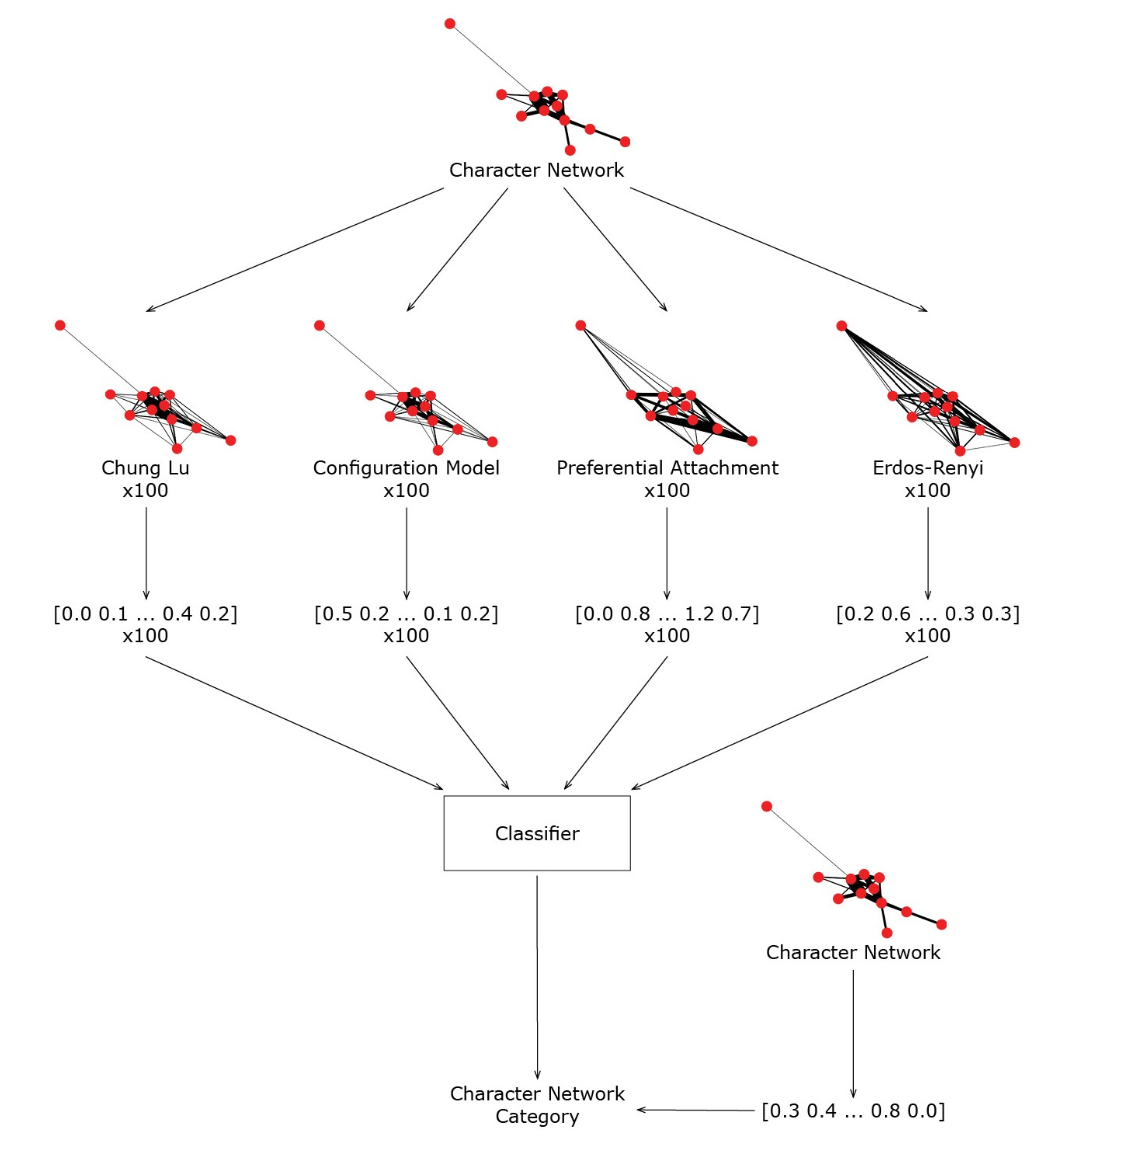
\includegraphics[width=1.0\textwidth]{Figures/PLOT.png}
\end{figure}

\newpage
\subsection{Tables}

\begin{table}[ht]
\centering
\caption{Multi-Graph Classifier Accuracies}
\begin{tabular}{|l|c|c|}
\hline
\textbf{Classifier Algorithm} & \textbf{Mean Training Accuracy} & \textbf{Mean Test Accuracy} \\ \hline
Support Vector Classifier     & 49.36\%                         & 46.69\%                     \\ \hline
AdaBoost                      & 66.28\%                         & 61.88\%                     \\ \hline
K-Nearest Neighbors           & \textbf{82.35\%}                & \textbf{72.67\%}            \\ \hline
Stochastic Gradient Descent   & 69.81\%                         & 67.38\%                     \\ \hline
\end{tabular}
\end{table}


\begin{table}[ht]
\centering
\caption{Directed Graph Classifier Accuracies}
\begin{tabular}{|l|c|c|}
\hline
\textbf{Classifier Algorithm} & \textbf{Mean Training Accuracy} & \textbf{Mean Test Accuracy} \\ \hline
Support Vector Classifier     & 57.27\%                         & 51.13\%                     \\ \hline
AdaBoost                      & 67.25\%                         & 64.38\%                     \\ \hline
K-Nearest Neighbors           & \textbf{90.11\%}                & \textbf{84.81\%}            \\ \hline
Stochastic Gradient Descent   & 81.67\%                         & 77.50\%                     \\ \hline
\end{tabular}
\end{table}

\begin{table}[ht]
\centering
\caption{Multi-Graph Character Network Labels}
\begin{tabular}{|l|c|}
\hline
\textbf{Graph Model}                     & \textbf{Proportion of Networks} \\ \hline
Multi-Graph Erdos-Renyi                  & 1.13\%                          \\ \hline
Multi-Graph Configuration Model          & 35.66\%                         \\ \hline
Multi-Graph Preferential Attachment      & \textbf{48.95\%}                \\ \hline
Multi-Graph Chung Lu                     & 14.26\%                         \\ \hline
\end{tabular}
\end{table}

\begin{table}[htbp]
\centering
\caption{Directed Character Network Labels}
\begin{tabular}{|l|c|}
\hline
\textbf{Graph Model}                     & \textbf{Proportion of Networks} \\ \hline
Directed Erdos-Renyi                  & 3.24\%                          \\ \hline
Fast Directed Reciprocal          & \textbf{49.92\%}                         \\ \hline
Directed Preferential Attachment      & 5.51\%                \\ \hline
Directed Chung Lu                     & \textbf{41.33\%}                        \\ \hline
\end{tabular}
\end{table}

\newpage
\subsubsection*{Acknowledgments}

I would like to express my deepest gratitude to Prof. Abhishek Samantray for his exceptional teaching, guidance, and practical insights into the domain of Network Systems. His course, HSN-619 (Social and Economic Networks), was both intellectually stimulating and deeply engaging.  

The lessons imparted during the course provided meaningful perspectives that enriched my understanding of the complex fabric of the world around us. Through his teaching, I developed a new lens to perceive people, entities, sentiments, and the intricate linkages connecting them. This transformative learning experience has broadened my horizon and encouraged me to explore network systems in greater depth.  

I am truly thankful for the opportunity to learn under his mentorship and for the valuable lessons that will continue to influence my academic and professional journey.

\subsubsection*{References}

\small{
[1] Agaev, R., \& Chebotarev, P. (2005). “On the spectra of nonsymmetric Laplacian matrices.” Linear Algebra and its Applications, 399, 157-168.

[2] Aparıcio, D., Ribeiro, P., \& Silva, F. (2015). “Network comparison using directed graphlets.” arXiv preprint arXiv:1511.01964.

[3] Bauer, F. (2012). “Normalized graph Laplacians for directed graphs.” Linear Algebra and its Appli- cations, 436(11), 4193-4222.

[4] Bonato, A., D’Angelo, D. R., Elenberg, E. R., Gleich, D. F., \& Hou, Y. (2016). “Mining and mod- eling character networks.” In Algorithms and Models for the Web Graph: 13th International Workshop, WAW 2016, Montreal, QC, Canada, December 14–15, 2016, Proceedings 13 (pp. 100-114). Springer Inter- national Publishing

[5] Burstein, D. (2017). “Asymptotics of the spectral radius for directed Chung-Lu random graphs with community structure.” arXiv preprint arXiv:1705.10893.

[6] Chung, F. (2006). “The diameter and Laplacian eigenvalues of directed graphs.” The Electronic Journal of Combinatorics, 13(1), N4. Chicago.

[7] Danescu-Niculescu-Mizil, C. (2011) “Movie Dialog Corpus.” [Dataset]. Retrieved from Kaggle.

\end{document}
